\documentclass[10pt]{article}
\setlength{\parskip}{0.25\baselineskip}
\usepackage[margin=1in]{geometry} 
\usepackage{amsmath,amsthm,amssymb, graphicx, multicol, array}
\usepackage[font=small,labelfont=bf]{caption}
\usepackage{tikz}
\usepackage{float}

\newcommand{\supp}{{\text{supp}}} 
\newcommand{\bv}{{\text{BV}}}
\newcommand{\ac}{{\text{AC}}}

\newenvironment{problem}[2][]{\begin{trivlist}
\item[\hskip \labelsep {\bfseries #1}\hskip \labelsep {\bfseries #2.}]}{\end{trivlist}}

\begin{document}
 
\title{Homework \#4}
\author{Eric Tao\\
Math 233: Homework \#4}
\maketitle

\begin{problem}{Question 1}

Let $L_1, L_2$ be lines in the plane. For which pairs of $L_1, L_2$ do there exists real functions, harmonic on the entire plane, 0 on $L_1 \cup L_2$, but not vanishing identically?

\end{problem}
\begin{proof}[Solution]

First, we notice that for any real function $v$, harmonic on the entire plane, it is the imaginary part of some holomorphic function. First, we know already that by 11.10, every real harmonic function is the real part of a holomorphic function, locally at least. Then, by considering disks around every point $z \in \mathbb{C}$, this can be extended to a holomorphic function $f$ such that $\Re(f) = v$, because on the disks, the local holomorphic functions may only differ by an imaginary constant, and it must align on intersections of disks, thus there may only be a single entire function.

Now, consider $i f$. Since $i$ is a constant, this is clearly holomorphic. Further, by construction $\Im(f) = v$. Thus, we have a holomorphic function such that $v$ is its imaginary part.

Now, suppose $v$ is harmonic, and $v(L_1) = 0, v(L_2) = 0$. Without loss of generality, since we may translate $v$ without affecting the derivatives, we may take $L_1 \cap L_2 = \{ (0,0)\}$. By a further linear change of coordinates, we may assume that $L_1$ is the real line, which will keep $v_{xx} + v_{yy} = 0$. 

Suppose $L_1$ and $L_2$ intersect.  Suppose that the angle between $L_1, L_2$ is $\theta_0$.

By the Schwarz reflection principle (11.14), and a relabeling of the two lines as need be, if we call $\sigma_1, \sigma_2$ the reflections of the plane with respect to $L_1, L_2$, we must have that $f(\sigma_1(z)) = \overline{f}(z), f(\sigma_2(z)) = \overline{f}(z)$. In particular then, on $L_1, L_2$, we have that $v(\sigma_1(z)) = v(z) = 0, v(\sigma_2(z)) = v(z) = 0$. Pictorially:

\begin{figure}[H]
\centering
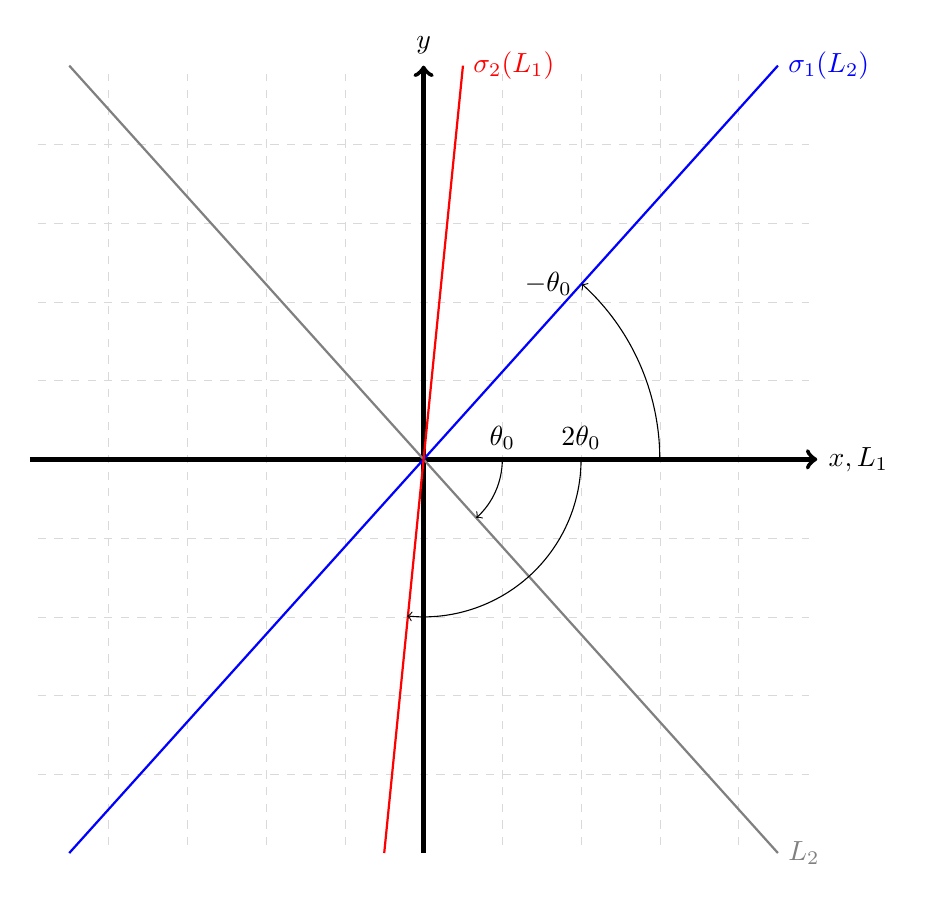
\begin{tikzpicture}
\draw[help lines, color=gray!30, dashed] (-4.9,-4.9) grid (4.9,4.9);
\draw[->,ultra thick] (-5,0)--(5,0) node[right]{$x, L_1$};
\draw[->,ultra thick] (0,-5)--(0,5) node[above]{$y$};
\draw[gray, thick] (-4.5,5) -- (4.5,-5) node[right]{$L_2$};
\draw[blue, thick] (-4.5, -5) -- (4.5, 5) node[right]{$\sigma_1(L_2)$};
\draw[red, thick] (-0.5, -5) -- (0.5, 5) node[right]{$\sigma_2(L_1)$};
\draw[black, ->] (1,0) node[above]{$\theta_0$} arc (0:-48:1) ;
\draw[black, ->] (2,0)  node[above]{$2\theta_0$} arc (0:-96:2);
\draw[black, ->] (3,0) arc (0:48:3)  node[left]{$-\theta_0$} ;
\end{tikzpicture}
\end{figure}

where we have that the angle between $L_1, \sigma_1(L_1)$ is $2 \theta_0$ because the angle between $\sigma_1(L_1)$ and $L_2$ is $\theta_0$, due to how reflections work. Further, we also see that $\sigma_1(L_2)$ takes on the angle $- \theta_0$.

We notice that we may iterate this process, and in fact generate lines of $k\theta_0$ via successive reflections. However, we know that if $\theta_0$ is not a rational multiple of $\pi$, then $\{ e^{im\theta_0} :m \in \mathbb{Z} \}$ is dense in $T$. And since $v = 0 $ on all of these lines, if it is $0$ on a dense set, then it is $0$ everywhere by continuity. Thus, this implies that we must have that $\theta_0$ is a rational multiple of $\pi$.

Now, suppose instead that $L_1, L_2$ are parallel. In such a case, applying the Schwarz reflection principle on successive lines, we note that then we must have that $v$ is periodic, $0$ at each interval $d = \text{dist}(L_1, L_2)$, since we can keep translating and applying reflections to find a line on the opposite side. For example, assuming $L_1: x = 1, L_2: x = 5$ one such $v$ could be $v(x,y) = e^{y} \sin(\pi(x-1)/\pi)$. This is generalizable with a suitable linear transformation on $x,y$ to match our parallel 1-D lattice.

\end{proof}

\begin{problem}{Question 2}

Suppose $\Delta$ is a closed equilateral triangle in the plane, with vertices $a,b,c$. Find $\max\{ |z-a||z-b||z-c| \}$ for $z \in \Delta$. 

\end{problem}

\begin{proof}[Solution]

\end{proof}

\begin{problem}{Question 3}

Suppose $f \in \mathcal{H}(\Pi^+)$, where $\Pi^+= \{ z = x + yi : y > 0 \}$, and $|f| \leq 1$. How large can $|f'(i)|$ be? Find the extremal functions.

\end{problem}

\begin{proof}[Solution]

First, for $U = \{ z : |z| < 1 \}$, we consider the map $\psi: U \to \Pi^+$ via:

$$\psi(z) = i \frac{1 - z}{1 + z} $$.

On $U$, this map is holomorphic. Further, this is injective. Suppose we have that $\psi(z) = \psi(w)$. Then, since on $U$, $z, w \not = -1$:

$$ i \frac{1 - z}{1 + z} = i\frac{1 - w}{1 + w} \implies (1 + w)(1 - z) = (1+ z)(1-w) \implies 1 + w - z - wz = 1 + z - w - wz \implies 2w = 2z \implies w = z$$

Further, we have that this map is surjective onto $\Pi^+$. Let $\zeta = a + bi \in \Pi^+$. Then, we have that, for $z = x + yi$:

$$ f(z) = \zeta \iff i \frac{1 - x - yi}{1 + x + yi} = a + bi \iff 1 - x - yi = -ai - axi + ay + b + bx + byi $$
$$ \iff \begin{cases} 1 - x = ay + b + bx \\ -y = -a - ax + by\end{cases} \iff x = \frac{1 - ay - b}{1 + b}$$

where we've used the fact that $z \in U$ so $1 + x + yi \not = 0$ and $\zeta = \Pi^+$, so $b \not = -1$. Now, substituting into the second equation, this would enforce that:

$$ -y = -a - a\frac{1 - ay - b}{1 + b} + by \iff -y\left(1 + b + \frac{a^2}{b+1}\right) = -a- \frac{a - ab}{1 + b} = \frac{-2a}{1 + b} \iff$$

$$ y = \frac{2a}{1 + b} \cdot \frac{b+1}{ a^2 + (b+1)^2} = \frac{2a}{a^2 + (b+1)^2} $$

Now, substituting back in for $x$, we find that:

$$ x  =  \frac{1 - a  \frac{2a}{a^2 + (b+1)^2} - b}{1 + b} = \frac{1}{1 + b} \cdot \frac{a^2 + (b+1)^2 - 2a^2 - a^2b - b(b+1)^2}{a^2 + (b+1)^2} = \frac{1}{b+1} \frac{-a^2(b+1) + (b+1)^2(1-b)}{a^2 + (b+1)^2}=$$
$$ \frac{ 1 - a^2 - b^2}{a^2 + (b+1)^2} $$

Now, we need only check that this lives within $U$. Well:

$$ x^2 + y^2 = \frac{1}{(a^2 + (b+1)^2)^2} [ (1 - a^2 - b^2)^2 + 4a^2] $$

It should be clear that this is always less than the denominator. If we expand everyyhing out, we see that we have the numerator as:

$$ 1 + a^4 + b^4 + 2a^2 - 2b^2 + 2a^2b^2 $$

and the denominator as:

$$ a^4 + 2a^2(b+1)^2 + (b+1)^4 = a^4 + 2a^2b^2 + 4a^2b + 2a^2 + b^4 + 4b^3 + 8b^2 + 4b + 1 $$

Subtracting the numerator from the denominator, we see:

$$ (a^4 + 2a^2b^2 + 4a^2b + 2a^2 + b^4 + 4b^3 + 8b^2 + 4b + 1) -  (1 + a^4 + b^4 + 2a^2 - 2b^2 + 2a^2b^2) = $$
$$ 4a^2b+ 4b^3+ 10 b^2 + 4b $$

Now, because $(a,b)$ are chosen from the upper half plane, we have that this number must be positive, since $a^2 \geq 0$, and $b > 0$. Thus, we have that $x^2 + y^2 < 1$, and therefore $z \in U$. Thus, $\psi$ is surjective.

Lastly, we consider the action of $\psi$ on $T = \{ z : |z| = 1 \}$, or really, $T \setminus \{ -1 \}$. Well, if $|z| = 1$, we may write it as $z = e^{i \varphi}$. First, we notice that:

$$\begin{cases} \sin(x) = \frac{e^{ix} - e^{-ix}}{2i} \\ \cos(x) = \frac{e^{ix} + e^{-ix}}{2} \end{cases} \implies \tan(x) = i \frac{e^{ix} - e^{-ix}}{e^{ix} + e^{-ix}} = i \frac{e^{2ix} - 1}{e^{2ix} + 1}$$

Then, we have that:

$$ \psi(e^{i\varphi}) = i \frac{1 - e^{i\varphi}}{1 + e^{i\varphi}} = -i \frac{ e^{i\varphi} - 1}{1 + e^{i\varphi}} = -i \cdot i \tan\left(\frac{\varphi}{2}\right) =  \tan\left(\frac{\varphi}{2}\right)$$

Since on $T \setminus \{ -1 \}$, $\varphi \in (-\pi, \pi)$, and on $x \in (-\pi/2, \pi/2)$, $\tan(x) \in (-\infty, \infty)$, $\tan(\varphi/2)$ covers the real line.

Now, let $f$ be as given, and consider the map $g = f \circ \psi: U \to \mathbb{C}$. Because $|f| \leq 1$ on the upper half plane, and the work we've done above, we have that $g \in \mathcal{H}^\infty(U)$, $\Vert g \Vert_\infty \leq 1$, and since $g$ is defined on $U$, we have that, as stated in 12.5, we may take $\alpha = 0 < 1$. Further, if $g(0) = \beta$, then we may assume that $| \beta | < 1$, as otherwise, by the maximum modulus principle, since $|g| \leq 1$ on $U$, this extends to the boundary by continuity. So, if $|g(0)| = 1$, then $g$ is constant everywhere and the derivative is 0.

Then, by the discussion in 12.5, we have that:

$$ |g'(0)| \leq 1 - | \beta |^2 $$

However, here, we notice that because $g = f \circ \psi$, $\psi(0) = i \frac{ 1 - 0}{ 1+ 0} = i$, so $g'(0) = f'(i), g(0) = \beta = f(i)$. 

Thus, restated in terms of $f$, we have that:

$$ |f'(i)| \leq 1 - | f(i)|^2 $$

Thus, we have two conditions to realize the maximum value here across all functions $f$. Firstly, we require $f(i) = 0$, and secondly, by Theorem 12.2, if $f(i)= \beta = 0$, then we have that $|g'(0)|  = 1$ occurs if and only if $g = \lambda z$, for some $\lambda \in \mathbb{C} : | \lambda | = 1$, that is, $f$ composed with $\psi$ acts as a rotation by some $\lambda$ on the unit disk $U$. 

This means that, we need only take an inverse to $\psi$, with some scale factor for the rotation, and a translation such that $f(i) = 0$. Well, I claim that $f(z) = \frac{iz + 1}{-iz + 1}$ acts as a left inverse to $\psi$:

$$ f\left(i \frac{1-z}{1+z}\right) = \frac{- \frac{1-z}{1+z} + 1}{ \frac{1-z}{1+z} +1} = \frac{ -1 + z + z + 1}{ 1-z + 1 + z} = \frac{2z}{2} = z$$

Further, we see that $f(i) = \frac{i^2 + 1}{-i^2 + 1} = \frac{0}{2} = 0$. So that part is all set.

Then, the maximal functions take on exactly the form $f_\lambda(z) = \lambda  \frac{iz + 1}{-iz + 1}$ for $\lambda \in \mathbb{C} : |\lambda| = 1$. 

\end{proof}

\begin{problem}{Question 4}

Suppose $f \in \mathcal{H}(\Omega)$. Under what conditions can $|f|$ have a local minimum in $\Omega$?

\end{problem}
 
\begin{proof}[Solution]

\end{proof}
  

\begin{problem}{Question 5}

(a) Suppose that $\Omega$ is a region, $D$ is a disc, $\overline{D} \subset \Omega$,$f \in \mathcal{H}(\Omega)$, non-constant, and $|f|$ is constant on $\partial D$. Prove that $f$ has at least one zero in $D$. 

(b) Find all entire functions $f$ such that $|f(z)|  =1 $ for all $|z| = 1$. 

\end{problem}

\begin{proof}[Solution]

\end{proof}

\end{document}